\documentclass[a4paper,12pt]{article}
\usepackage[a4paper,top=2.0cm, bottom=1.5cm, left=1.5cm, right=1.5cm]{geometry}

\usepackage[T2A]{fontenc}			
\usepackage[utf8]{inputenc}		
\usepackage[english,russian]{babel}	
\usepackage{amsmath,amsfonts,amssymb,amsthm,mathtools} 
\usepackage{wasysym}
\usepackage{graphicx}
\usepackage{wrapfig}
\DeclareGraphicsExtensions{.pdf, .png, .jpg}
\graphicspath{{}}


\begin{document}


\section{Fashion Retrieval via Graph Reasoning Networks on a Similarity Pyramid}

\begin{wrapfigure}{r}{0.5\linewidth}
	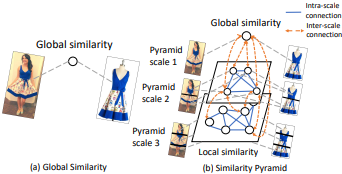
\includegraphics[scale = 1.1]{GRNet_intro.png}
\end{wrapfigure}
Авторы предлагают GRNet – модель для определения похожести элементов одежды, которая использует несколько представлений каждой картинки в разном масштабе, в отличие от более ранних моделей, использовавших единственное векторное представление. Модель вычисляет скор близости между соответствующими представлениями, а потом осуществляет message passing по полному графу, вершинами которого являются вычисленные скоры. Таким образом предлагается вычислять итоговую близость объектов и использовать ее для рекомендательной системы.\\

Математика:\\
$\{x_l^i \in \mathbb{R}^{C\times 1}\}$ и $\{y_l^i \in \mathbb{R}^{C\times 1}\}$ векторные представления $i$-го локального признака в $l$ масштабе. Для каждого масштаба $l$ и номеров признаков $i$ и $j$ считается вектор локальной близости $s_l^{ij}$:
$$s_l^{ij} = \frac{P|x_l^i-y_l^j|^2}{\|P|x_l^i-y_l^j|^2\|_2}$$
где $P$ -- проекционная матрица, снижающая размерность. Из этих векторов составляется итоговый граф (пирамида). Далее для каждой пары вершин $s_{l_1}^{ij}$ и $s_{l_2}^{mn}$ определяется скаляный вес $w_p^{l_1ijl_2mn}$:
$$w_p^{l_1ijl_2mn} = \frac{\exp((\mathbf{T}_{out}s_{l_1}^{ij})^\intercal(\mathbf{T}_{in}s_{l_2}^{mn}))}{\sum\limits_{l,p,q}\exp((\mathbf{T}_{out}s_{l_1}^{ij})^\intercal(\mathbf{T}_{in}s_{l}^{pq}))}$$ 
Тогда для $l_1=l_2$ это веса внутри одного масштаба, а для $l_1\neq l_2$ -- между разными, что позволяет им "сообщаться". Таким образом мы определили граф близости $G = (\mathbb{N},\mathbb{E})$, где $\mathbb{N} = \{s_l^{ij}\}$ а $\mathbb{E} = \{w_p^{l_1ijl_2mn}\}$.\\
Далее вектора в каждой вершине обновляются по следующему правилу:
$$\widehat{s}_{l_1}^{ij} =ReLU\left(W \sum\limits_{l_2,m,n}w_p^{l_1ijl_2mn}s_{l_2}^{mn}\right)$$


\section{Dressing as a Whole: Outfit Compatibility Learning Based on Node-wise Graph Neural Networks}
Авторы рассматривают задачи поиска подбора подходящего недостающего элемента одежды и оценки совместимости предложенного образа, используя граф, в котором каждая вершина есть категория элемента одежды, а каждый образ есть подграф. 

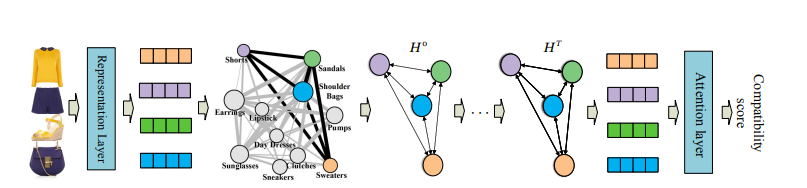
\includegraphics[scale = 0.87]{Dressing as a whole intro.png}\\

Математика:\\
Рассматривается множество образов $\mathcal{S} =\{s_1,s_2,\dots\}$ и множество элементов одежды $\mathcal{V} = \{v_1,v_2,\dots\}$. Для каждого элемента $v_i$ $f_i$ -- вектор его признаков $f_i$ а его представление в латентном пространстве $r_i$. Каждый $v_i$ также принадлежит некоторой категории $c_i$. Вершина графа соответствующая категории $c_i$ -- $n_i$, ее состояние -- $h_i$. Множество всех $n_i$ объединяется в граф $\mathcal{G} = (\mathcal{N}, \mathcal{E})$. Веса каждого ребра определяются как:
$$w(n_i, n_j) = \frac{Count_{c_i,c_j}/Count_{c_j}}{\sum_k Count_{c_i,c_k}/Count_{c_k}}$$
где $Count_{c_i,c_j}$ -- частота совместной встречаемости категорий $c_i$ и $c_j$, а $Count_{c_i}$ -- категории $c_i$.\\
Скрытые состояния вершин инициализируются как 
$$h_i^0 = tanh(r_i) = tanh(W_h^i f_i)$$
После инициализации следует несколько шагов взаимодействия вершин. На шаге $t$ вершина $i$ получает функцию всех своих соседей следующего вида:
$$a_i^t = \sum\limits_{n_j\to n_i \in \mathcal{E}} A[n_i, n_j]W_\rho h_j^{t-1} + b_\rho$$
где $W_\rho$ и $b_\rho$ -- веса и смещение общего для всех ребер линейного преобразования, $A$ -- матрица смежности вида:
$$A[n_i, n_j] = \begin{cases}
	w(n_i, n_j), if~n_i \to n_j \in \mathcal{E}\\
	0, else
\end{cases}$$
Чтобы сделать взаимодействие уникальным для каждой пары вершин, но не вводить уникальные матрицы для каждого ребра, вводятся 2 матрицы для каждой вершины $W_{out}^i, W_{in}^j$, а матрица $W_rho$ для каждого ребра $n_i\to n_j$ заменяется на:
$$W_\rho^{n_i\to n_j} = W_{out}^i W_{in}^j$$
Далее происходит преобразования состояния вершины $n_i$ вида:
$$~z_i^t = \sigma(W_za_i^t + U_zh_i^{t-1} + b_z)$$
$$~r_i^t = \sigma(W_ra_i^t + U_rh_i^{t-1} + b_r)$$
$$~~~~~~~~~~~~~~~\tilde{h}_i^t =tanh(W_ha_i^t + U_h(r_i^t \odot h_i^{t-1}) + b_h)$$
$$h_i^t = \tilde{h}_i^t\odot z_i^t + h_i^{t-1}(1-z_i^t)$$
где $W_z, W_r, W_h, b_z, b_r, b_h$ -- обучаемые параметры, $z_i^t$ и $r_i^t$ -- "gate" и "reset gate" векторы соответственно. Указанная процедура повторяется $T$ раз.\\
Наконец, после $T$ рекуррентных шагов для получения итогового скора применяется $self-attention$ над всеми вершинами графа.




\section{Fashion Outfit Complementary Item Retrieval}
Скукотень какая-то, придумали лосс, который почти триплет, но не триплет, и делают свертки.


\section{Hierarchical Fashion Graph Network for Personalized Outfit Recommendation}
Авторы статьи предлагают кроме совместимости образа рассматривать также консистентность предложений с предпочтениями пользователя. Для этого предлагается построить граф с иерархической структурой из 3-х уровней: уровень пользователя, уровень образов и уровень элементов одежды.

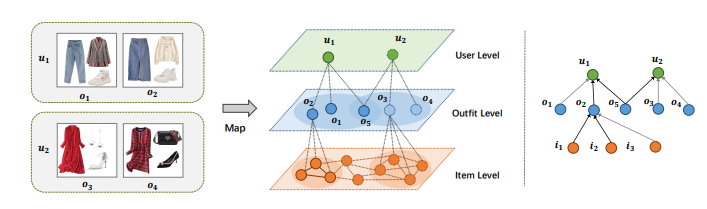
\includegraphics[scale = 0.97]{FashionGraphNet_intro.png}\\

На каждом из трех уровней эмбединги последовательно взаимно уточняются с помощью. \\
Математика -- буквально свертки с нелинейностями и усреднения 


\section{OutfitTransformer: Learning Outfit Representations for Fashion Recommendation
}
Авторы предлагают использовать архитектуру трансформера для обучения информативного представления образа целиком. Полученное представление используется для оценки совместимости образа, восстановления образа с пропущенными элементами и рекомендации подходящих вещей. Помимо изображений элементов одежды, авторы также используют их текстовое описание и одновременно тренируют 2 энкодера для текстового и графического представления каждого объекта.

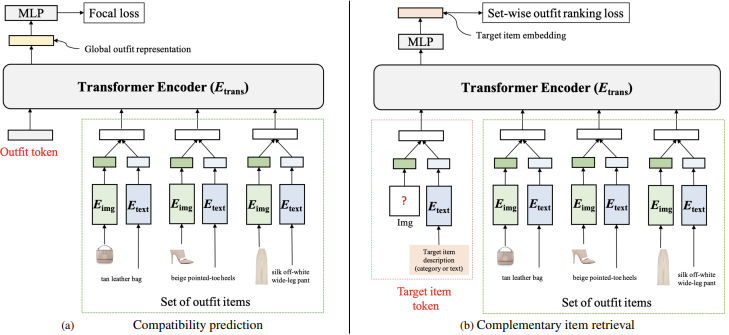
\includegraphics[scale = 0.8]{OutfitTransfromer intro.png}\\

Стоит заметить, что подход к использованию трансформера в данном случае не совсем традиционный: позиционное кодирование не используется, поскольку каждый элемент в образе равноправен, а значит операции в модели должны быть инвариантны к их перестановке (так это же снова граф!).

Обучают сначала в левом сетапе (оценка совместимости), а потом дообучают под правый (подбор подходящих элементов на основании эмбединга образа). Для левого используется focal loss. Для правого "set-wise outfit ranking loss" следующего вида: 
$$L(t, p, N) = L(t, p, N)_{All} + L(t, p, N)_{Hard}$$
$$L(t, p, N)_{All} = \frac{1}{|N|}=\sum\limits^{|N|}_{j=1}[d(t,f^p) - d(t, f_j^N)+m]_{+}$$
$$L(t, p, N)_{Hard} = \frac{1}{|N|}=\sum\limits^{|N|}_{j=1}[d(t,f^p) - \min\limits_{j=1\dots|N|}(t, f_j^N)+m]_{+}$$
где $t$ -- выход линейной сети после трансформера, $f^p$ -- позитивный пример (выбран из готового образа, оставшаяся часть которого пропускается через трансформер), $f^N$ для $L(t, p, N)_{All}$ -- негативные примеры случайно насемпленные из всего датасета, для $L(t, p, N)_{Hard}$ -- hard-negative-ы насемпленные из узких неподходящих к образу категорий, $m$ -- margin, $[..]_+$ -- hinge-loss.

\section{FAME-ViL: Multi-Tasking Vision-Language Model for\\ Heterogeneous Fashion Tasks}
Авторы изучают вопрос обучения мультимодальной модели сразу на несколько задач связанных с образами. Предложенная модель с помощью специфических адаптеров, превосходит все существовавшие подходы на каждой рассматриваемой задаче по отдельности.

\begin{wrapfigure}{l}{0.5\linewidth}
	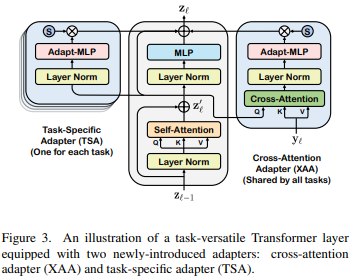
\includegraphics[scale = 1.0]{FAME-ViL_acrhitecture.png}
\end{wrapfigure}

Основой архитектуры предложенной модели выступает претренированный CLIP -- мультимодальный трансформер для текстовой и визуальной информации. Для того, чтобы приспособить модель к выполнению различных задач рекомендации, распознавания и оценки образов авторы предлагают 2 вида адаптеров: TSA -- Task-Specific Adapter для обучения специфическим для каждой задачи особенностям и XAA -- Cross-Attention Adapter для обеспечения возможности взаимодействиями между различными модальностями, общий для всех задач. Для TSA предлагается ввести дополнительные линейные слои (AdaptMLP) после каждого self-attention блока параллельно с основными:
$$z_l^{tsa}=s \cdot AdaptMLP(LN(z'_l))$$
где $s$ -- Обучаемый множитель.\\
В XAA используется дополнительный Multi-Head Cross Attention (MHXA) с группой линейных слоев после него:
$$z_l^{xaa} = s\cdot AdaptMLP(LN(MHXA(z_l',y_l)))$$
где $y_l$ выход self-attention слоя части сети для другой модальности.\\
Далее полученные $z_l^{tsa}$ и $z_l^{xaa}$ аггрегируются с обычным выходом следующим образом:
$$z_l = MLP(LN(z_l')) + z_l'+z_l^{tsa}+\epsilon\cdot z_l^{xaa},~\epsilon\in\{0,1\}$$
$\epsilon$ -- барьерный множитель включающий или выключающий определенный адаптер для определенной задачи. 

Рассматриваемая архитектура обучается на разные задачи в трех режимах Contrastive, Fusion и Generative с различными используемыми адаптерами и функциями потерь. 

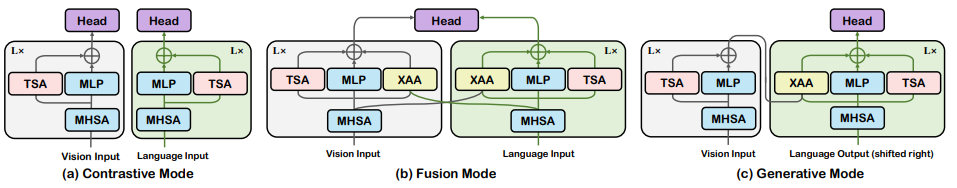
\includegraphics[scale = 0.7]{FAME-ViL_modes.png}

\begin{itemize}
	\item[]\textbf{Contrastive mode:}\\
	Этот режим используется для кросс-модальных рекомендаций (XMR) (текст по картинке/картинка по тексту). Все XAA блоки отключены. Обучение производится на выборках пар картинка-текст $(\textbf{I}, \textbf{T}) = \{(I_1, T_1), \dots, (I_B, T_B)\}$, сначала они по отдельности проходят через части сети для соответствующей модальности, потом с помощью контрастной функции потерь производится максимизация схожести выходов этих частей.
	$$\mathcal{L}_{XMR} = \frac{1}{2} [\mathcal{L}_{InfoNCE}(\mathbf{T}, \mathbf{I}) + \mathcal{L}_{InfoNCE}(\mathbf{I}, \mathbf{T})]$$
	$$\mathcal{L}_{InfoNCE} = -\frac{1}{B}\sum\limits_{i=1}^{B}\log\frac{\exp(s(X_i, Y_i)/\tau)}{\sum_{j=1}^B\exp(s(X_i, Y_j)/\tau)}$$
	где $\tau$ -- обучаемая (???) температура. $s$ -- симметричная функция схожести $s(I_i, T_j) = f_\theta^{[c]}(I_i)^T\cdot f_\theta^{[c]}(T_j)$, где $f_\theta^{[c]}$ -- собственно нейросеть.
	\item[]\textbf{Fusion mode:}\\
	Используется для субкатегориального распознавания (SCR) и направляемых текстом рекомендаций (TGIR). И XAA, и TSA блоки включены. \\
	Задача SCR -- предсказание подкатегории для данного товара, основываясь на тексте и картинке. Исходя из специфики задачи, к выходу сети дополнительно добавляется классификатор, cross-entropy-loss которого и минимизируется:
	$$\mathcal{L}_{SCR} = -\mathbb{E}_{(I,T)\sim D}\log P\left(f_\theta^{[f]}(I, T)\right)$$
	Для TGIR подход немного другой, поскольку необходимо получить представления отдельно для исходной картинки с текстовым промптом и целевой картинки, поэтому для $(\mathbf{I^r}, \mathbf{T})$ соответственно исходных картинок и текстовых запросов сеть запускается в $fusion$ режиме, а для целевых изображений $I^t$ в $contrastive$ режиме. Далее считается контрастная функция потерь вида
	$$\mathcal{L}_{TGIR} = \mathcal{L}_{InfoNCE}((I^r,T), I^t)$$
	
	\item[]\textbf{Generative mode:}\\
	Используется, например, для генерации подписей к картинкам в авторегрессионном режиме. TSA блоки включены в обеих модальностях, XAA -- только image-to-text. Причем часть обрабатывающая входное изображение используется как энкодер, а вторая -- как декодер. Функция потерь классическая для seq2seq трансформера.
\end{itemize}

Кроме упомянутого интересно, что авторы используют идею Multi-Teacher Distillation для обучения модели на все задачи одновременно. Для начала они обучают модель такой же архитектуры на каждую задачу в отдельности, а потом дистиллируют знания всех обученных моделей в одну.





		
\end{document}